\section{Introduction}\label{intro}\sloppy


Data cleaning is widely recognized as a major challenge in almost all forms of data analytics~\cite{nytimes}, and analysts may spend upwards of 80\% of the analysis effort to clean and prep the data.  A common form of data errors are those where attribute values are incorrect---these errors can vary from missing data, incorrect or biased values, misspellings, the concatenation of multiple attributes due to extraction errors, and more.  These errors must be fixed because they can affect the output of downstream applications (e.g., SQL queries, visualizations, ML models).  Thus, developing automated data cleaning techniques can greatly reduce the end-to-end data analysis process.

\begin{figure}[t]
  \centering
 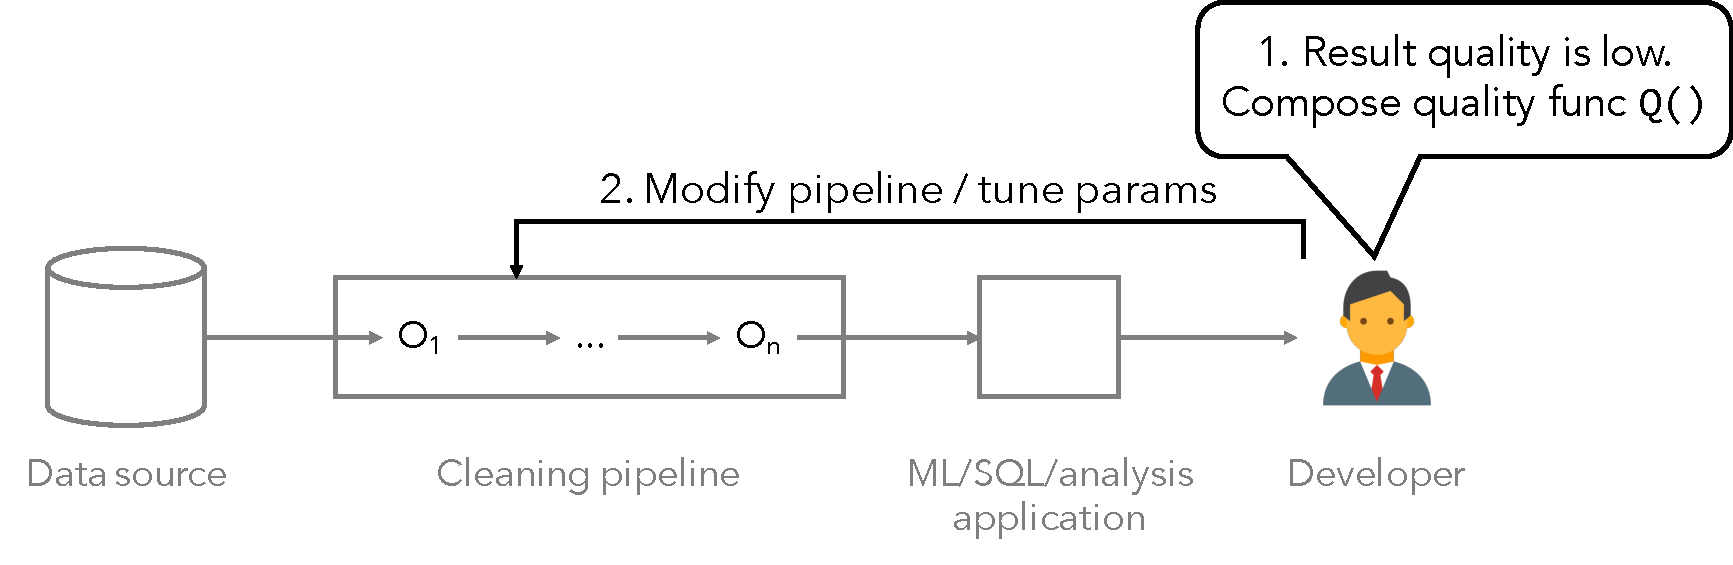
\includegraphics[width=\columnwidth]{figures/user-pipeline}
 \caption{\small Typical data cleaning pipeline.  The user finds that analysis results (of SQL query, ML model, web application, etc) are suspicious and iteratively (1) composes a quality function to characterize the suspicious quality issues, and (2) modifies the data cleaning pipeline to address the errors.  The bottleneck is the human-in-the-loop.  \label{fig:user-pipeline}}
\end{figure}

\ewu{Introduce data quality as separate from the cleaning plan.}
Data cleaning is challenging because the {\it data quality measure}, which defines a quantitative objective for a data cleaning system, as well as the {\it physical cleaning plan}, which is the sequence of data transformations needed to most improve the data quality measure, are rarely known ahead of time. Instead, data quality issues arise as part of developing the application and cleaning the data~\cite{krishnan2016hilda}.  

% For example, the developer in Figure~\ref{fig:user-pipeline} analyzes CS department sizes at different schools and finds many departments with only one faculty member.  At this point,  Based on her domain expertise, she must 1) characterize the data quality issues that affect the application results, and 2) create or modify her data cleaning pipeline to fix those errors. 

\ewu{Human in the loop, and issues with specialized systems}
This iterative pattern makes data cleaning a human-in-the-loop problem, where the developer explores a large space of data quality issues {\it and} data cleaning programs.  A number of data cleaning systems have been developed to automate parts of this process.  Specialized data cleaning systems (e.g., HoloClean~\cite{}, XXX~\cite{}, etc~\cite{}) are designed to search for cleaning programs for specific types of data quality issues (e.g., value errors in HoloClean, or data extraction errors in Wrangler~\cite{}).  Thus, if the user finds that her data quality issues are applicable to such a system, then she can tune the system \ewu{DESCRIBE HOW} and run it.  
\ewu{Issues with pipeline systems}
Unfortunately, many datasets contain a mixture of error types~\cite{} that require combining different data cleaning systems or operators.  End-to-end cleaning pipelines (e.g., Wisteria, XXX, YYY) address this by implementing extensible libraries of data cleaning operators, and providing APIs to parameterize and combine the operators into cleaning pipelines.  Although these systems make it easier to construct and execute a pipeline, the space of possible operator pipelines and parameterizations of each operator is exponential in the number of operators, parameters, and pipeline depth, and is infeasible for developers to manually search.

This paper proposes to tackle the human-in-the-loop data cleaning problem by developing techniques to automatically generate and tune data cleaning pipelines based on user-specified quality characteristics.  Thus, the user can primarily focus on composing and expressing data quality issues, and allow the system to explore the space of physical cleaning plans.  The search procedure is progressive, in the sense that it quickly generates acceptable cleaning plans, and refines those plans over time.  Thus, the user can immediately assess her hypothesis, or test multiple hypotheses in parallel.

This approach present two technical challenges. First, it requires a simple way to express quality function so that it can both describe input data errors {\it as well as the downstream application output}, and be efficient to evaluate.   
To this end, we model data quality as a function $Q(\mathcal{D}) \in [0, 1]$ over the dataset $\mathcal{D}$ that returns $1$ if there are no discernable quality issuues, lower values correspond to a dirtier table. We further provide a library that translates common classes of data errors such as functional constraint violations, outliers, and statistical inconsistencies into efficient quality functions.


The second challenge is to search the space of cleaning plans to maximize the data quality function.  A naive approach is to leverage \emph{hyperparameter tuning} for machine learning~\cite{li2017hyperband, sparks2017keystoneml, baylor2017tfx, golovin2017google, liaw2018tune}, which identifies the optimal assignment of hyperparemeters to maximize an objective function (e.g., training accuracy for ML models).   For a pipeline of up to $k$ cleaning operators, we can create a parameter that represents the operator type in each of the pipeline slots, along with additional operators to tune each operator in each pipeline slot.  A hyperparameter tuning algorithm will then select and parameter a sequence of operators.

Although this approach is possible, it ignores important aspects of data cleaning problems that can enable more efficient and flexible approaches.  First, the parameter space is exponential in the pipeline depth, the types of operators, and the number of parameters to tune each operator.   This makes block-box approaches a very difficult discrete optimization problem.   Second, it is difficult to know up front how many operators are needed in the pipeline, thus tuning $k$ can be challenging: the optimization problem is too difficult if $k$ is too large, but an effective cleaning pipeline may not exist if $k$ is too small.  Finally, a subtle challenge is that existing black-box search algorithms do not explicitly reason about interactions between pipeline components, and can end up in local maxima or waste considerable resources searching redundant parameter combinations. %  , and those effects are latently captured in the parameter space and accuracy metric.

% In contrast, data cleaning programs are often a sequence of transformations applied one after the other, thus the entire space of hyperparameters does not need to be learned jointly\ewu{Is this really true?  Are we making a correctness argument or an efficiency argument?}. 

% Second, the transformations are not commutative, and prior transformations can affect subsequent transformations.  For example, data extraction must happen before type inference can be effective. This means that local decisions need to account for how they may affect later transformations.  Third


\begin{figure}[t]
\centering
 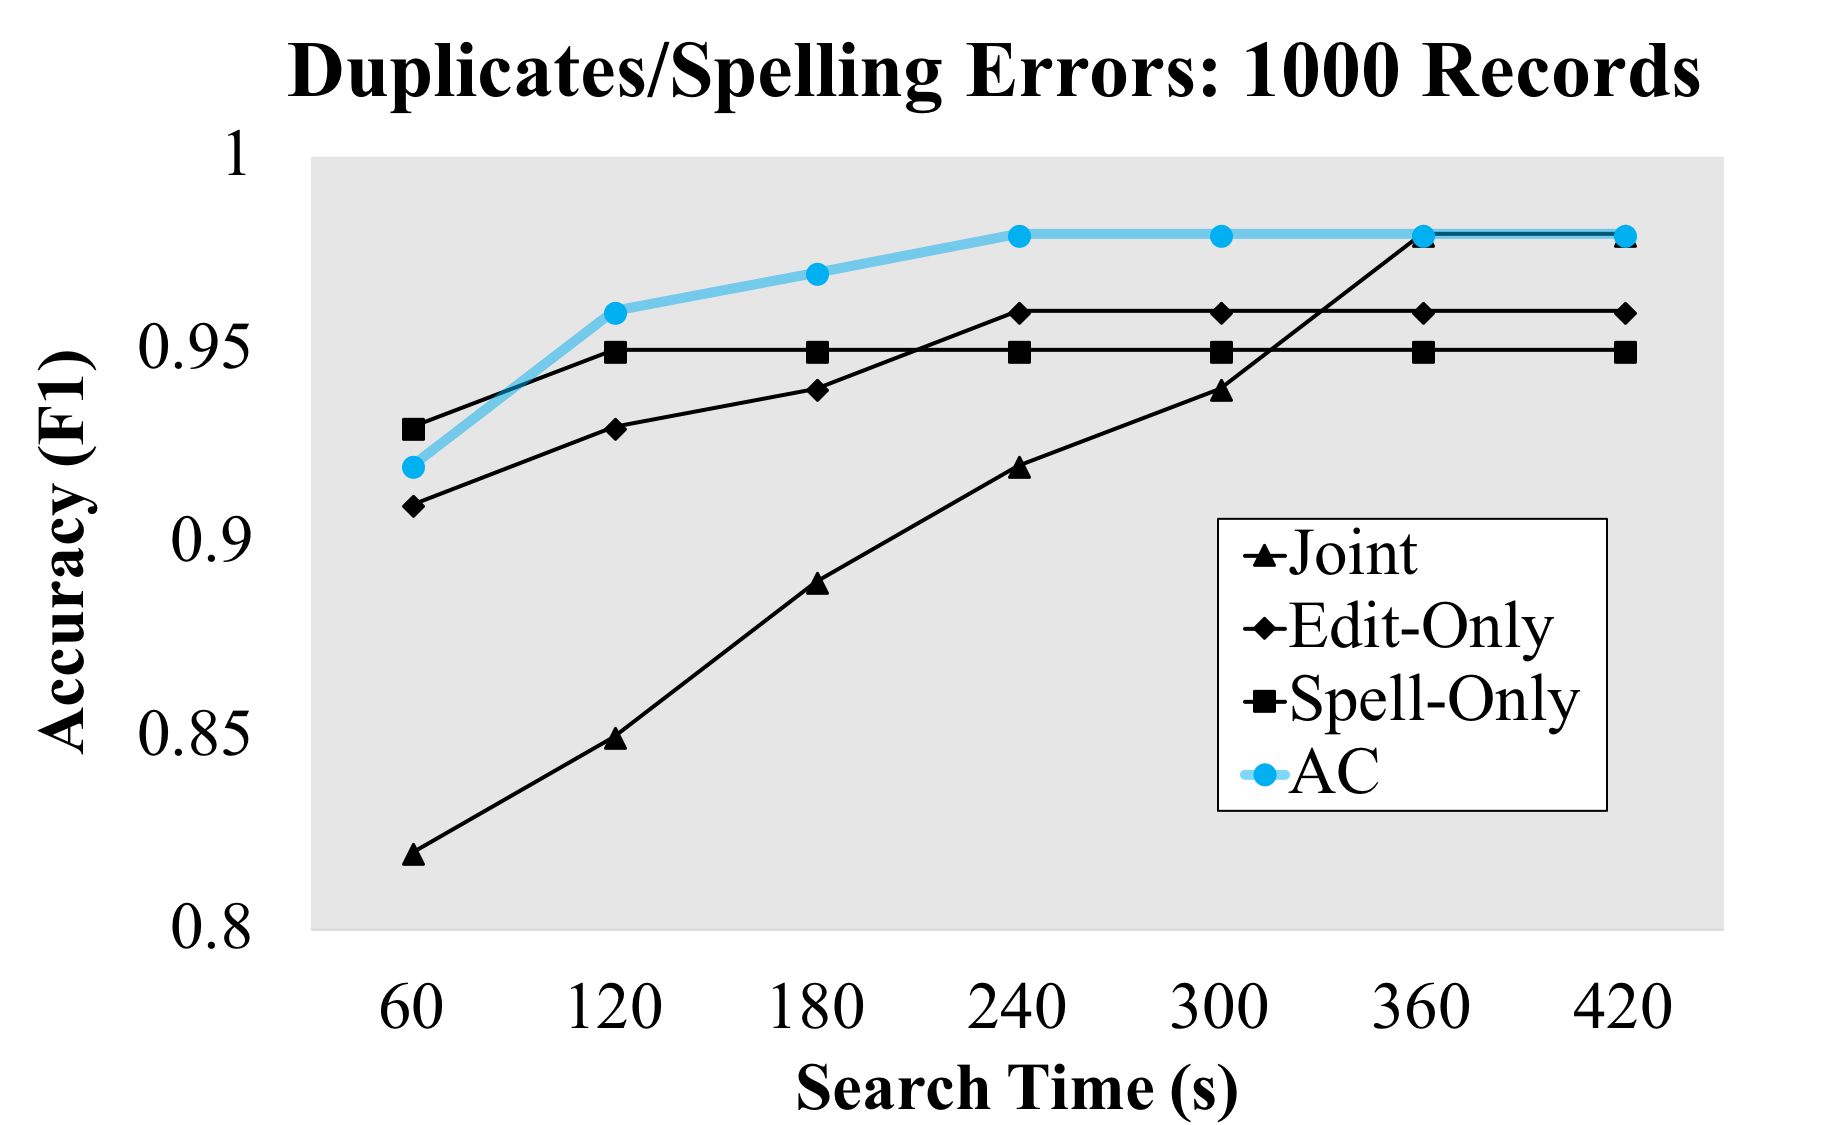
\includegraphics[width=0.9\columnwidth]{figures/teaser-experiment.png}
 \caption{\small 10\% of a dataset of dictionary words are duplicated with randomly generated spelling errors. The dataset is to be cleaned with a similarity matcher and a spell checker. Holistically, tuning the parameters of both with \textsf{python hyperopt} (BB-Full) is inefficient due to interactions between the two data cleaning options. It takes over 3x the amount of search time for the joint optimization to exceed the best tuned single cleaning method (BB-Edit and BB-SpellCheck) \label{fig:teaser}}
\end{figure}

To illustrate these points, Figure~\ref{fig:teaser} evaluates hyperparameter search based on \ewu{XXX}~\cite{}\footnote{Implemented using \textsf{python hyperopt}} for a toy data cleaning problem.  We corrupted 1000 dictionary words so that 10\% are duplicated with randomly generated spelling errors affecting 1-3 characters. The quality function is the F1 score of the cleaned dataset as compared to the ground truth.  We consider two parameterized operators: \texttt{edit\_dist\_match(thresh)} is a string edit distance similarity matcher with a tunable threshold, and \texttt{ispell(rec)} is a spell checker with a tunable recommendation parameter based on the distance between the dictionary word and the misspelled word.  The two operators partially overlap in their cleaning behavior, and we will see how it affects the search problem below.   

We compare hyperparameter search for three fixed pipelines:  single-operator pipelines (\texttt{edit\_dist\_match}) and (\texttt{ispell}), and a joint pipeline (\texttt{edit\_dist\_match}, \texttt{ispell}).  By fixing the operator pipeline, the search algorithm only needs to learn parameterizations of the operators.  Although we expect the joint pipeline to perform the best, Figure \ref{fig:teaser} shows that there is a trade-off between runtime and data quality (measured as F1 score).  It takes 3$\times$ amount of search time for the joint pipeline to exceed the best single-operator pipeline.    In contrast, the single operator pipelines quickly converge to an F1 score of $\ge95\%$.  The reason is because the two operators overlap in functionality (some duplicates can be fixed by \texttt{ispell} or \texttt{edit\_dist\_match}), which forces the join optimization to explore redundant parameter settings that have the same cleaning results.  In practice, pipelines and the set of operators can be much larger, thus the likelihood of redundant operators, or even operators that reverse changes made by previous operators, is high.


% Our paper 1) encodes cleaning objectives as a quality function, and provides tools for users to compose quality functions easily, 2) models cleaning as a sequential learning problem, 3) uses machine learning to dynamically prune the search space during the search process.  

To address this search problem, we treat pipeline generation and tuning as a greedy tree-search problem.   Each path is a candidate data cleaning pipeline whose quality can be evaluated by running the pipeline over the input dataset and running the quality function.  The benefit is that the search can be easily parallelized across candidate paths as well as partitions of the dataset.  To accelerate the search process and prune unpromising paths, we dynamically learn a model that predicts the expected quality of a given cleaning pipeline.  This model thus avoids the need to execute the pipeline and quality function in order to evaluate a given path.    We use periodic synchronization to update the prediction model across parallel searches.  \ewu{We can describe it this way, but we should just call it reinforcement elarning and introduce + adopt the terminology.}

We have implemented this search framework in a system called \sys.  \sys is initialized with a library of parameterized data cleaning operators.  Similar to recent systems such as HoloClean~\cite{rekatsinas2017holoclean}, each operator specifies its repairs as attribute value assignments.  The user composes a quality function by using a pre-exising library of quality specifications, or writing a custom Python function over the dataset or application output.  \sys then executes the tree-search algorithm and progressively improves the best cleaning pipeline explored so far.  

\noindent Our contributions include:
\begin{itemize}[leftmargin=*, topsep=0mm, itemsep=0mm]
  \item Explicitly decoupling automated data cleaning into a data quality function and operator search procedure.  Users can focus on refining the data quality function.  Further, users can easily add new operators for the system to consider.
  \item A progressive data cleaning system based on tree-search that quickly generates acceptable cleaning pipelines, and improves the pipeline over time.   
  % \item Rethinking parameter optimization in data cleaning and data transformation with a novel candidate-search framework called \sys. \sys includes an API for specifying data cleaning operations as well as accuracy metrics.
  \item A suite of pragmatic optimizations, such as fast pruning using predictive models, multi-node parallelization, and data sharing to reduce network communication bottlenecks, that reduce the runtime by \ewu{XXX$\times$}.
  \item A systematic study of the benefits and limitations of \sys in terms of data cleaning accuracy (precision, recall), and the runtime.  We show that \sys can solve incremental refinements of the data quality measure $yyy\times$ faster than from scratch, and that \ewu{SOME OTHER FINDING}
\end{itemize}


